\chapter{Arquitectura de un robot delta}\label{CAP3}

\section{Funcionamiento general}

La principal tarea de un robot es ir de un punto a otro para realizar determinada acción. Para realizar la tarea se debe pasar por una serie de pasos con el fin de asegurar la ejecución exitosa de dicha tarea. Con el fin de explicar brevemente los pasos a seguir para lograr dicho objetivo, en la figura \ref{f:Cap3-1_diagrama_de_flujo_robot_accion} se muestra un ejemplo básico de un diagrama de flujo de un robot delta accionado por motores paso a paso.\\

Los pasos del diagrama de flujo son los siguientes:

\begin{itemize}
    \item Definir los puntos de inicio y final de la trayectoria del robot.
    \item Elegir el tipo de trayectoria, posiciones, velocidades y aceleraciones impuestas y no dañar los componentes del robot.
    \item Comprobar la cinemática y dinámica para asegurar la trayectoria impuesta y no dañar los componentes del robot.
    \item Transformación de la trayectoria cartesiana al espacio articular de los actuadores que controlan el movimiento de las partes mecánicas del robot.
    \item Traducción de trayectoria en el espacio articular a pulsaciones que entiendan los drivers de cada motor.
    \item Envío de pulsos al driver de los motores por medio de un controlador.
\end{itemize}

        \newpage

    \begin{figure}[h]
        \centering
        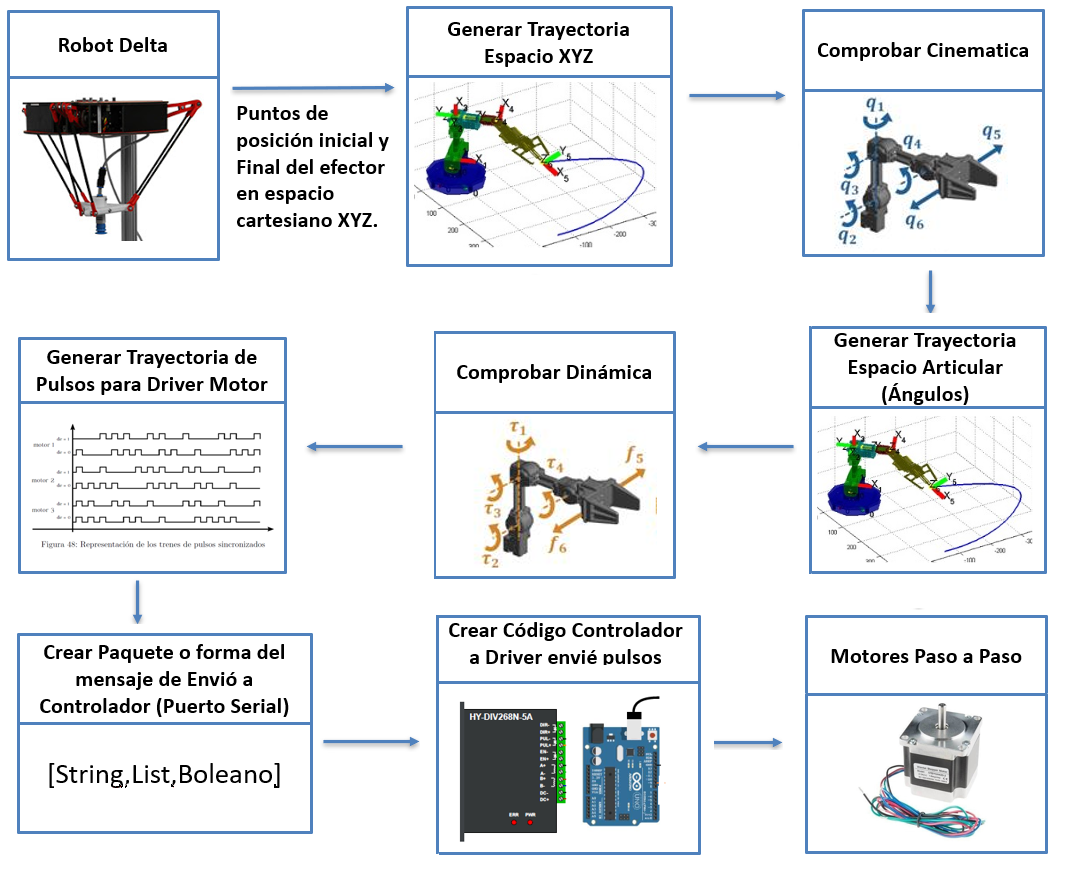
\includegraphics[width=1.0\linewidth]{Main/Chapter3/Images3/3-1/diagrama-de-flujo-robot.png}
        \caption{asd}
        \label{f:Cap3-1_diagrama_de_flujo_robot_accion}
    \end{figure}

        \newpage
\section{Estructura de un robot delta}
%00X0 : reordenar los títulos del cap al diagrama de abajo en formato general, y luego explicar los software específicos para nosotros

    El robot delta puede ser subdivido por categorías de acuerdo al grupo estructural al que pertenezcan. Estas categorías facilitan la generación de conceptos para cada grupo de manera independiente \cite{Robot_parelelo_tipo}
    
    \begin{figure}[h]
        \centering
        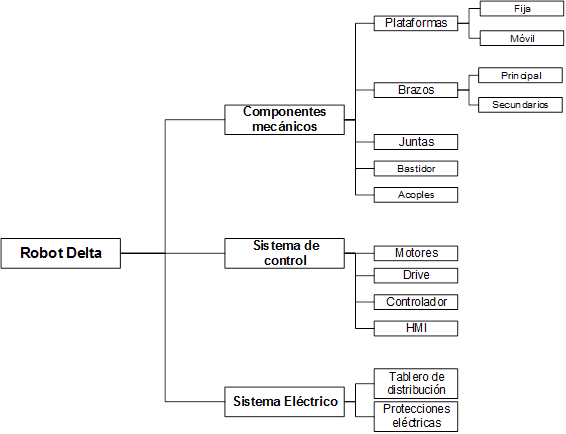
\includegraphics[width=0.85\linewidth]{Main/Chapter3/Images3/3-2/esquema-categorias-estructura.png}
        \caption{asd}
        \label{f:Cap3-2_esquema_arquitectura_robot_delta}
    \end{figure}
    
    \begin{enumerate}
        \item{ \textbf{Los componentes mecánicos}: son todas las piezas físicas que componen el robot delta. Es muy importante la elección del tipo de juntas a elegir ya que restringen el espacio de trabajo del robot delta. Por otro lado, se pueden optimizar las dimensiones de los largos de los brazos y antebrazos del robot con respecto a la energía suministrada a los motores y al espacio de trabajo.}
        \item{\textbf{El sistema de control}: es todo lo que está relacionado con el control del movimiento del robot delta. Los motores, que mueven los brazos del robot delta, deben controlarse a través de drivers por la complejidad de su accionamiento.}
        \item{ \textbf{El controlador}: puede tener el algoritmo que cree las trayectorias cartesianas para realizar el movimiento del robot de un punto a otro. El HMI es la interfaz que ayuda a visualizar si el movimiento deseado del robot es correcto antes de que se realice.}
        \item{   \textbf{Los componentes eléctricos}: son todo lo relacionado con la electricidad como fuentes de poder para los motores, cables de conexión, fusibles, switch, etc.}
    \end{enumerate}

        \newpage

    Con la intensión de modelar la arquitectura de un robot delta como guía para el desarrollo de este trabajo, se crea una arquitectura con ejemplos reales enfocado solo en el sistema de control, tal como se presenta en la figura \ref{f:Cap3-2_esquema_sistema_control} donde:

    \begin{figure}[h]
        \centering
        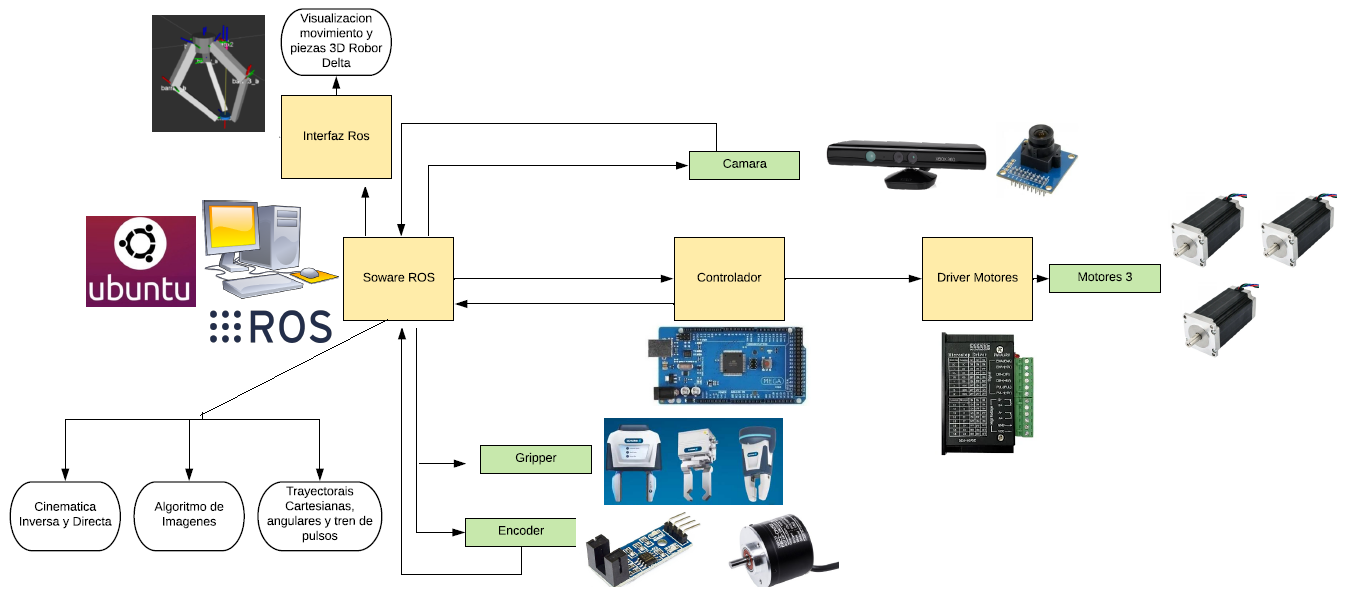
\includegraphics[width=1\linewidth]{Main/Chapter3/Images3/3-2/sistema-de-control.png}
        \caption{asd}
        \label{f:Cap3-2_esquema_sistema_control}
    \end{figure}
    
    \begin{itemize}
        \item \textbf{Software ROS:} Es el encargado de procesar y ejecutar los algoritmos de cinemática y dinámica del robot delta. Además, controla el envió, la recepción y el procesamiento de datos de los sensores y el controlador.
        \item \textbf{Controlador:} Realiza la conversión de la trayectoria cartesiana o angular a un formato compatible con el driver de los motores. Se puede utilizar Arduino, Raspberry Pi, etc.
        \item \textbf{Rviz:} Es la interfaz gráfica que simula las trayectorias del robot.
        \item \textbf{Kinect:} Sensor RGB y de profundidad que controla la posición del robot creando un lazo cerrado.
        \item \textbf{Actuadores:} Motores paso a paso controlados por drivers.
        \item \textbf{Encoder:} Sensor de velocidad y posición angular que controla los actuadores creando un lazo cerrado.
        \item \textbf{Gripper:} Pinzas qe sujetan los objetos.
    \end{itemize}
    
    Para controlar a un alto nivel cada punto anterior, se necesita de mucho estudio, investigación y práctica, por lo que en esta tesis solo abarcara lo relacionado con el Software ROS y la interfaz gráfica Rviz.  
    
    \newpage

    
\section{Partes mecánicas (hay que repensar esto)}
    Con el fin de describir el robot delta, en esta sección se presenta un resumen del capítulo 2 de la tesis doctoral del ingeniero mecánico Reymond Clavel, el creador de este mecanismo, realizada en École Polytechnique Fédérale de Lausanne [referencia tanto]. 

    
    \subsection{Investigación}
    El primer objetivo que busca Reymond Clavel es el movimiento de piezas ligeras a gran velocidad en robots, ya que las aplicaciones objetivo de su investigación se encuentran en los campos del envasado en el sector alimentario, despaletización y paletización al inicio o al final de una línea de montaje, el montaje de componentes mecánicos, etc. Para todas estas operaciones se requiere un ritmo alto de producción/operación y los contactos de la industria de Clavel confirmaban esa tendencia en aquellos tiempos.
    
    Para lograr una alta tasa de trabajo durante operaciones que requieren carreras reducidas, el robot debe tener esencialmente una capacidad de aceleración y frenado; esta propiedad se obtiene mediante el uso de potentes actuadores debajo y mediante una estructura móvil muy ligera. Un estudio anterior de robot rápido del Clavel hizo posible probar el uso de gatos hidráulicos a alta velocidad con masas relativamente pesadas, pero por razones de coste y limpieza no querían utilizar energía hidráulica por lo que lo llevo al enfoque de una ``estructura móvil y ligera``.
    
    La búsqueda de un concepto se basó en una metodología enseñada en estudios de microtecnología en EPFL. Según la metodología antes mencionada, el primer paso de la cadena de costos consiste en definir la función global del producto considerado. La representación mediante una caja negra con las diferentes entradas y salidas sintetiza efectivamente esta información.
    
    \begin{figure}[htb]
        \centering
        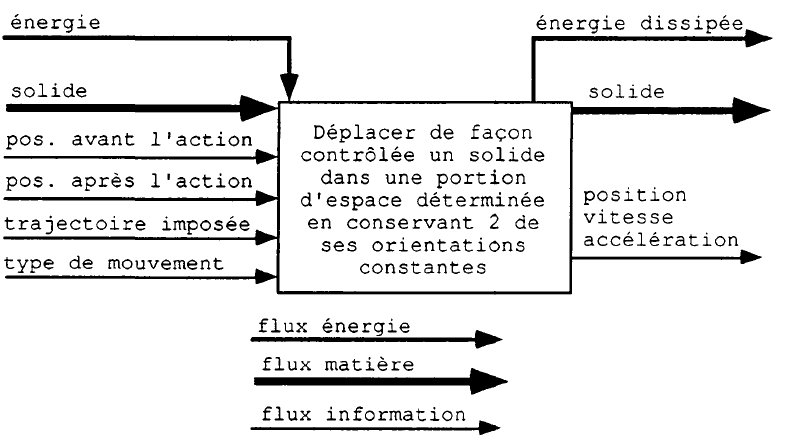
\includegraphics[width=0.8\linewidth]{Main/Chapter3/Images3/3-3/caja-negra-reymond.png}
        \caption{asd}
        \label{f:Cap3-3_caja_negra_reymond}
    \end{figure}
    
    \newpage
    
    \subsection{Elección del concepto ``Delta``}
    El catálogo de soluciones del anexo A2.2 de la tesis doctoral [tanto] presenta 18 tipos de soluciones principales que permiten mantener constantes 2 orientaciones de un sólido. La figura 2.3 muestra las soluciones más interesantes para el objetivo previsto. Entre estas 18 soluciones, Reymond conserva aquellas que tienen las siguientes particularidades:

     \begin{figure}[htb]
        \centering
        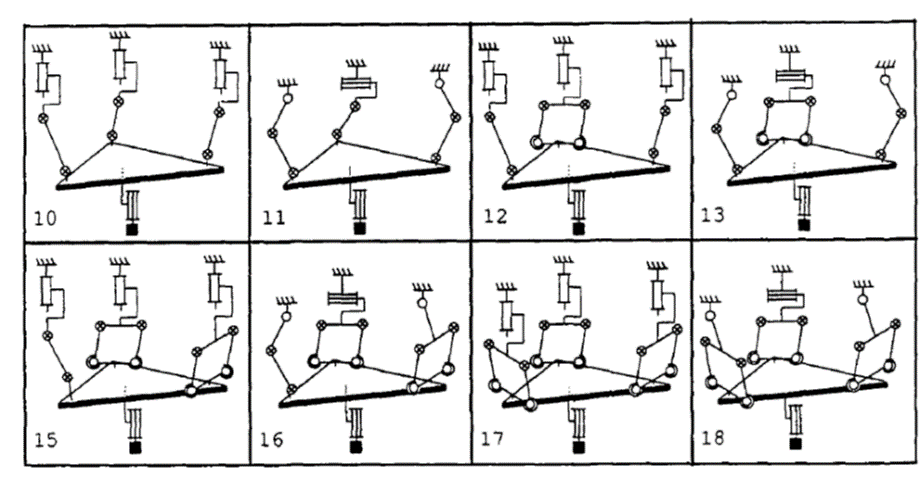
\includegraphics[width=0.85\linewidth]{Main/Chapter3/Images3/3-3/soluciones-interesantes.png}
        \caption{Extracto de las soluciones más interesantes del catálogo del Apéndice A.2.2}
        \label{f:Cap3-3_soluciones_interesantes_catalogo}
    \end{figure}
    
    \begin{enumerate}
        \item El movimiento en el espacio (con tres grados de libertad) es proporcionado por el tres actuadores asegurados a la base fija, las soluciones 10 a 13 y 15 a 18 de la figura \ref{f:Cap3-3_soluciones_interesantes_catalogo} cumplen esta condición.
        \item Los actuadores son del tipo giratorio. Las soluciones 11, 13, 16 y 18 cumplen esta condicion.
        \item La estabilidad del órgano terminal está asegurada por una mayoría de elementos que trabajan en tensión-compresión más que en torsión. Finalmente se adopta la solución numero 18.
    \end{enumerate}
    
     \begin{figure}[htb]
        \centering
        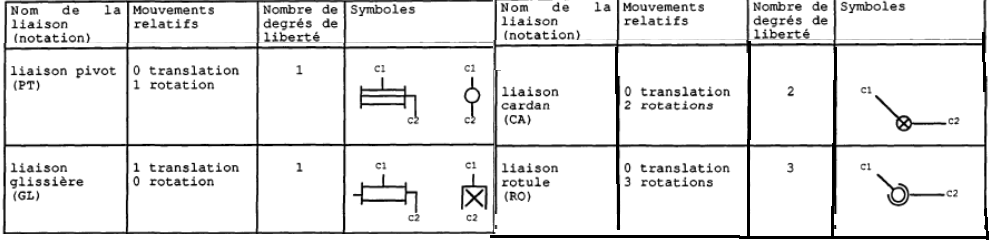
\includegraphics[width=0.9\linewidth]{Main/Chapter4/Images4/juntas.png}
        \caption{Extracto de las soluciones más interesantes del catálogo del Apéndice A.2.2}
        \label{f:Cap3-3_soluciones_interesantes_catalogo_JUNTAS}
    \end{figure}
    
        \newpage
    
    \subsection{Descripción del concepto ``Delta'' y sus componentes}
    La figura \ref{f:Cap3-3_esquema_principal_robot_delta} sirve de apoyo para la descripción del robot DELTA y su funcionamiento. Este es un robot con cuatro grados de libertad. Se compone principalmente de una ``base fija'' (1) integrada a un marco de soporte de la instalación y una placa móvil (5); el nombre que se le da a esta última pieza es ``góndola'' (nacelle en frances). La conexión entre la base fija (1) y la góndola (5) se realiza mediante tres cadenas cinemáticas, cada una de ellas está formado por un ``brazo'' (2) montado en una articulación pivotante sobre la base fija y 2 ``barras paralelas'' (3) provistas cada una de una articulación (4) en cada extremo. El conjunto anterior que forma 2 barras paralelas y 2 elementos de conexión al brazo y a la góndola, se denomina ``paralelogramo''. Cada brazo (2) es impulsado por un ``motor de brazo'' (7) que, con mayor frecuencia, adopta la forma de un conjunto de motor reductor de sensor. La ``Pinza'' (10) del motor (6), a través del ``eje telescópico'' (8) provisto de una articulación tipo cardan (9) tiene oculto uno de sus extremos.

    \vspace{-1em}

    % Multiples imagenes        
    \begin{figure}[h]
         \centering
              \subfloat[Esquema principal del robot delta]{
               \label{f:Cap3-3_esquema_principal_robot_delta}
                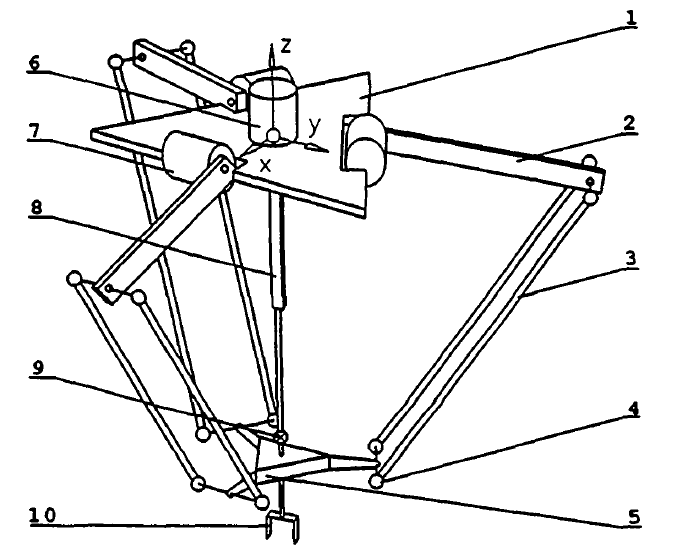
\includegraphics[width=0.5\textwidth]{Main/Chapter3/Images3/3-3/esquema-principal-robot-delta.png}}
              \subfloat[Representación de paralelogramos del robot delta]{
               \label{f:Cap3-3_ayuda_dimensiones}
                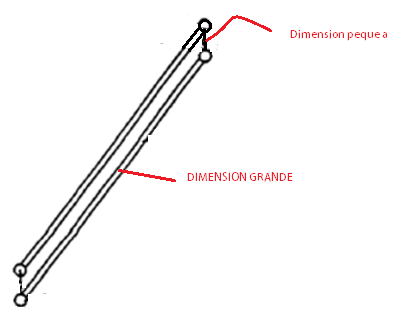
\includegraphics[width=0.5\textwidth]{Main/Chapter3/Images3/3-3/ayuda-dimensiones.png}}
         \caption{Múltiples imágenes}
         %\label{f:animales}
    \end{figure}

    La orientación de la góndola está asegurada constantemente por los 3 paralelogramos que comprenden cada uno 2 dimensiones pequeñas y 2 dimensiones grandes formadas por las barras paralelas. Cada lado pequeño integrado al extremo de un brazo permanece constantemente paralelo al eje de rotación del brazo en cuestión. Los 3 pares de barras paralelas aseguran que las 3 pequeñas dimensiones integradas a la góndola permanezcan paralelas a las pequeñas dimensiones integradas a los extremos de los brazos, por tanto, paralelas a los ejes de rotación de los brazos que, por construcción, se ubican en el mismo plano. Las juntas en los extremos de las barras paralelas son del tipo de junta esférica, por lo que cada barra puede girar alrededor de su eje longitudinal; esta rotación no altera el comportamiento de esta estructura articulada que forma el paralelogramo del espacio. Una conexión por resortes y estribos entre las 2 barras paralelas simplifica la construcción de las rótulas y limita las evoluciones giratorias de las barras paralelas.
    
    \newpage

\section{Software Robor Operating System (ROS)}
    
    En esta sección se proporciona una descripción general de Robot Operating System, por sus siglas ROS y sus principales lineamientos. ROS es un marco para desarrollar software de robótica. El software está estructurado bajo un paradigma modular, pequeños paquetes que se comunican entre si mediante rápidos mensajes. Este paradigma se fomenta la reutilización de código y la colaboración global por sobre los entornos particulares.
    
    \begin{figure}[htb]
        \centering
        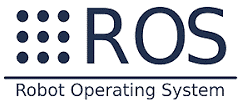
\includegraphics[width=0.5\linewidth]{Main/Chapter3/Images3/3-4/logo-ros.png}
        \caption{Logotipo de ROS}
        \label{f:Cap3-4_logo_ros}
    \end{figure}
    
    \subsection{Historia}
    
        ROS es un gran proyecto que tiene muchos antepasados y contribuyentes. Mucha gente en la comunidad de investigación robótica sintió la necesidad de un marco de colaboración abierto. Varios proyectos en la Universidad de Stanford a mediados de la década de 2000 involucraban inteligencia artificial incorporada e integradora, como el Stanford AI Robot (STAIR) y el programa Personal Robots (PR), que crearon prototipos internos de los tipos de sistemas de software dinámicos y flexibles como lo es ROS. Se basó en Switchyard, que era parte de un proyecto de STAIR y fue escrito por Morgan Quigley en Stanford. En 2007, Willow Garage, Inc., una incubadora de robótica cercana, proporcionó importantes recursos para extender estos conceptos mucho más y crear implementaciones bien probadas. Desde el 2013 hasta el presente, ROS es mantenido permanentemente por la OSRF (Open Source Robotics Foundation) de Google y desde el 2017 cambio su nombre a Open Robotics.
        
        \begin{figure}[htbp]
            \centering
            \subfigure{
\includegraphics[width=40mm]{Main/Chapter3/Images3/3-4/entidade-asociadas-al-inicio-de-ros-1.png}}
            \subfigure{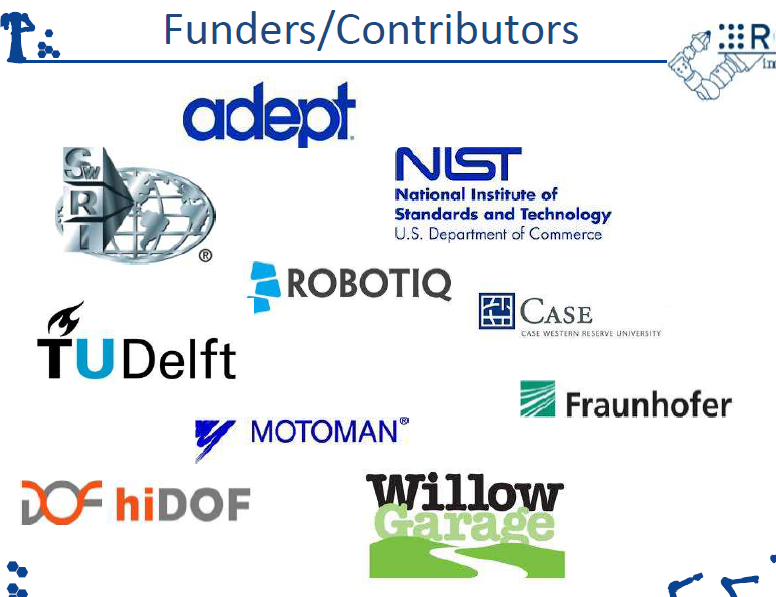
\includegraphics[width=60mm]{Main/Chapter3/Images3/3-4/entidade-asociadas-al-inicio-de-ros-2.png}}
            \subfigure{
\includegraphics[width=40mm]{Main/Chapter3/Images3/3-4/entidade-asociadas-al-inicio-de-ros-3.png}}
            \caption{Entidades asociadas al inicio de ROS} 
            \label{f:Cap3-4_entidades_inicio_ros}
        \end{figure}
        
        La mayoría de las compañías y laboratorios de investigación en robótica están ahora portando su software a ROS. Esta tendencia también es visible en robots industriales, donde compañías están paulatinamente migrando de aplicaciones propietarias a ROS. El movimiento llamado ROS Industrial se ha incrementado en estos últimos años y su objetivo, básicamente, consiste en extender las capacidades avanzadas de ROS a la automatización y la robótica industrial. Este proyecto comenzó como un intento de colaboración de Yaskawa Motoman Robotics, Southwest Research Institute (SwRI) y Willow Garage. En enero de 2012, Shaun Edwards de SwRI fundó un software repositorio, alojado en Github, donde la comunidad robótica puede encontrar interfaces para manipuladores industriales, pinzas, sensores y redes de dispositivos.
        
        
        Finalizando con la breve historia de ROS, se puede decir que se utiliza en estos momentos en todo el mundo en instituciones académicas, industriales y de investigación. Los desarrolladores han contribuido con miles de paquetes, incluidas soluciones de algunos de los principales expertos del mundo en áreas específicas. Las nuevas empresas de robots ofrecen interfaces ROS con sus productos, y las empresas de robots industriales establecidas también están introduciendo interfaces ROS. Con la adopción generalizada de ROS como el enfoque estándar de facto para la programación de robots, existe una nueva esperanza de acelerar las capacidades de los robots.

    \subsection{Que es ROS}
       ROS es una abreviatura de  Robot Operating System y es una plataforma de desarrollo de aplicaciones en robótica que provee estilos de programación (en particular, que se basa en nodos distribuidos y acoplados libremente); definiciones de interfaz y paradigmas para las comunicaciones entre nodos ; definiciones de interfaz para la incorporación de bibliotecas y paquetes; una colección de herramientas para visualización, depuración, registro de datos y diagnóstico del sistema; un repositorio de código fuente compartido; y puentes a múltiples bibliotecas útiles e independientes de código abierto.
       
       El objetivo principal de ROS es apoyar la reutilización de código en la investigación y el desarrollo de robótica. ROS es un marco distribuido de procesos (también conocido como nodos) que permite que los ejecutables se diseñen individualmente y se acoplen libremente en tiempo de ejecución. Estos procesos se pueden agrupar en paquetes, que se pueden compartir y distribuir fácilmente. ROS también es compatible con un sistema federado de repositorios de código que también permite la distribución de la colaboración. Este diseño, desde el nivel del sistema de archivos hasta el nivel de la comunidad, permite decisiones independientes sobre el desarrollo y la implementación, pero todos pueden combinarse con las herramientas de infraestructura ROS.
       
       ROS no es un sistema operativo convencional como Windows, Linux y Android en el sentido tradicional de gestión y programación de procesos; más bien, es un meta-sistema operativo que se ejecuta en el sistema operativo. ROS es un middleware, que proporciona los servicios que esperaría de un sistema operativo, incluida la abstracción de hardware, control de dispositivos de bajo nivel, implementación de funciones de uso común, transmisión de mensajes entre procesos y administración de paquetes. También proporciona herramientas y bibliotecas para obtener, compilar, escribir y ejecutar código en varios equipos.
       
        \begin{figure}[htb]
            \centering
            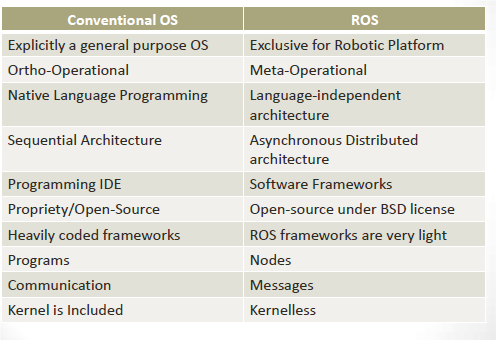
\includegraphics[width=0.8\linewidth]{Main/Chapter3/Images3/3-4/diferencia-ROS-SO.png}
            \caption{Diferencias entre un sistema operativo convencional y ROS}
            \label{f:Cap3-4_diferencias_ros_so}
        \end{figure}
        
        Las principales características de ROS se pueden resumir de la siguiente manera:
        
        \begin{itemize}
            \item \textbf{Plumbing:} ROS proporciona una infraestructura de mensajería de publicación y suscripción diseñada para respaldar la construcción rápida y sencilla de sistemas informáticos distribuidos.
            \item \textbf{Herramientas} ROS proporciona un amplio conjunto de herramientas para configurar, iniciar, introspectar, depurar, visualizar, registrar, probar y detener sistemas informáticos distribuidos.
            \item \textbf{Capacidades} ROS proporciona una amplia colección de bibliotecas que implementan funcionalidades robóticas útiles, con un enfoque en la movilidad, la manipulación y la percepción.
            \item \textbf{Ecosistema:} ROS es apoyado y mejorado por una gran comunidad, con un fuerte enfoque en la integración y documentación. ros.org es una ventanilla única que busca y aprende sobre los miles de paquetes ROS que están disponibles a través de desarrolladores de todo el mundo.
        \end{itemize}
        
        \begin{figure}[htb]
            \centering
            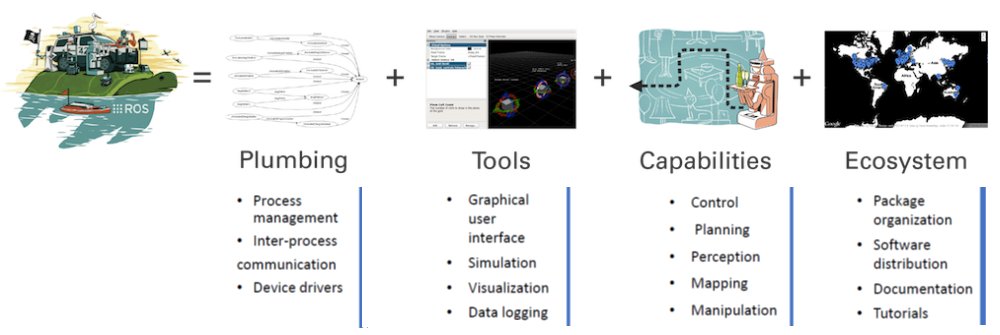
\includegraphics[width=1.0\linewidth]{Main/Chapter3/Images3/3-4/caracteristicas-ros.png}
            \caption{Principales características de ROS}
            \label{f:Cap3-4_caracteristicas_ros}
        \end{figure}
        
        Como se describe en la figura \ref{f:Cap3-4_caracteristicas_ros}, ROS es un sistema de apoyo para controlar un robot y sensor con una abstracción de hardware y desarrollar una aplicación de robot basada en sistemas operativos convencionales existentes.
        
        Un ejemplo se muestra en la Figura 2-2, la comunicación de datos ROS es compatible no solo con un sistema operativo, sino también con múltiples sistemas operativos, hardware y programas, lo que lo hace muy adecuado para el desarrollo de robots donde se combinan varios hardware. 
        
        \begin{figure}[htb]
            \centering
            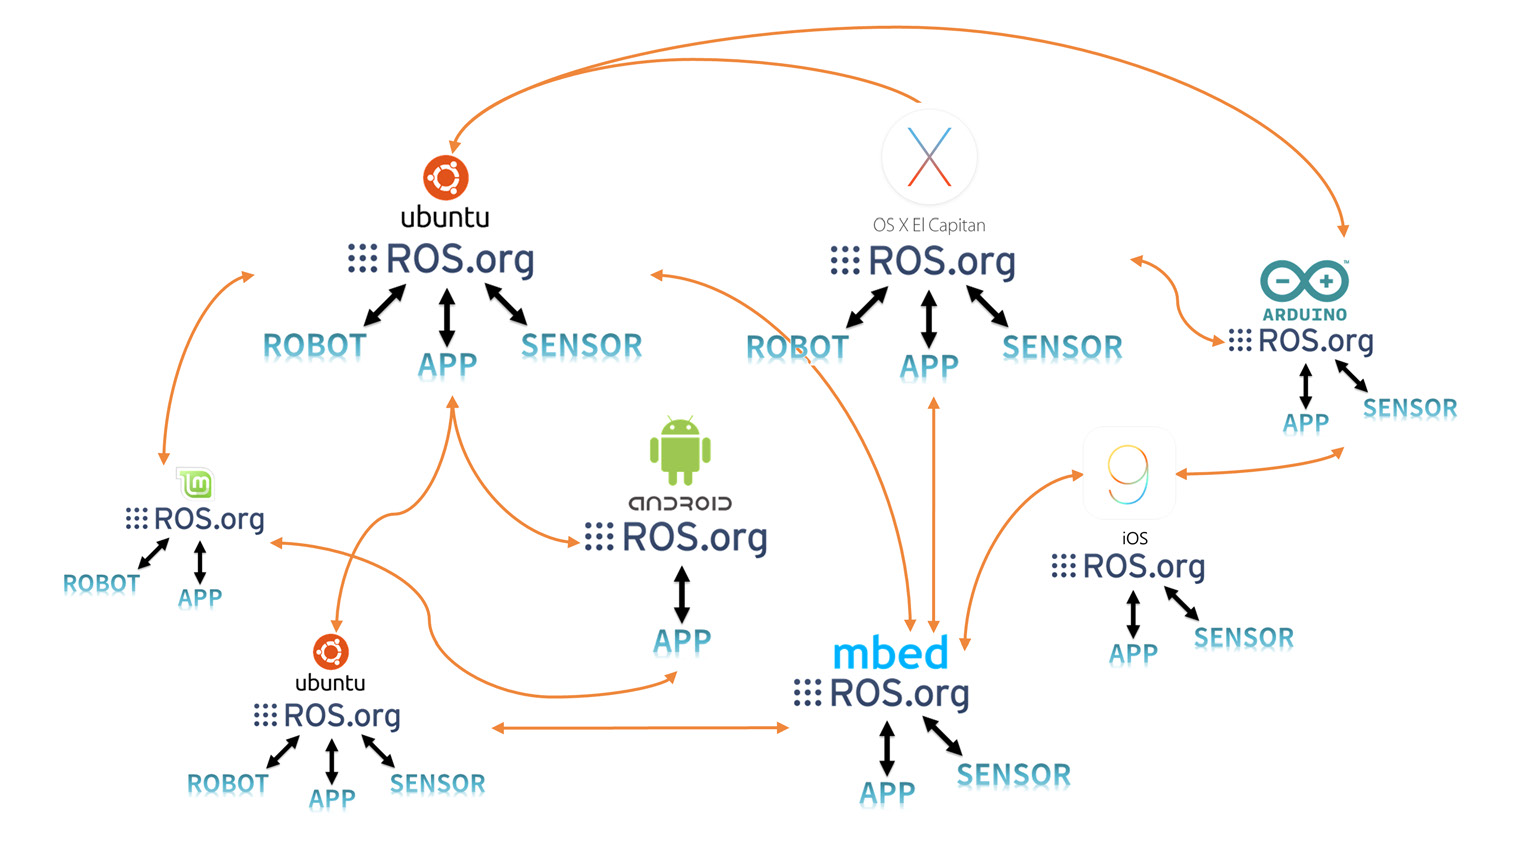
\includegraphics[width=0.9\linewidth]{Main/Chapter3/Images3/3-4/compatibilidad-ros.png}
            \caption{Compatibilidad de ROS y otras plataformas}
            \label{f:Cap3-4_compatibilidad_ros}
        \end{figure}
        
    \subsection{Objetivos de ROS}
    
        Todos los marcos de software imponen sus filosofías de desarrollo a sus colaboradores directa o indirectamente, a través de sus modismos y prácticas comunes. En términos generales, ROS sigue la filosofía de desarrollo de software de Unix en varios aspectos clave. Esto tiende a hacer que ROS se sienta ``natural'' para los desarrolladores que provienen de Unix, pero algo ``críptico'' al principio para aquellos que han utilizado principalmente entornos de desarrollo gráfico en Windows o Mac OS X. Los siguientes párrafos describen varios aspectos filosóficos de ROS.
        
        \subsubsection{Peer to peer (Nodos)}
        
            Los sistemas ROS consisten en numerosos programas pequeños de computadora que se conectan entre sí e intercambian mensajes continuamente. Estos mensajes viajan directamente de un programa a otro; no hay un servicio de enrutamiento central. Aunque esto hace que la ``plumbing'' subyacente sea más compleja, el resultado es un sistema que escala mejor a medida que aumenta la cantidad de datos.
            
            \begin{figure}[htb]
                \centering
                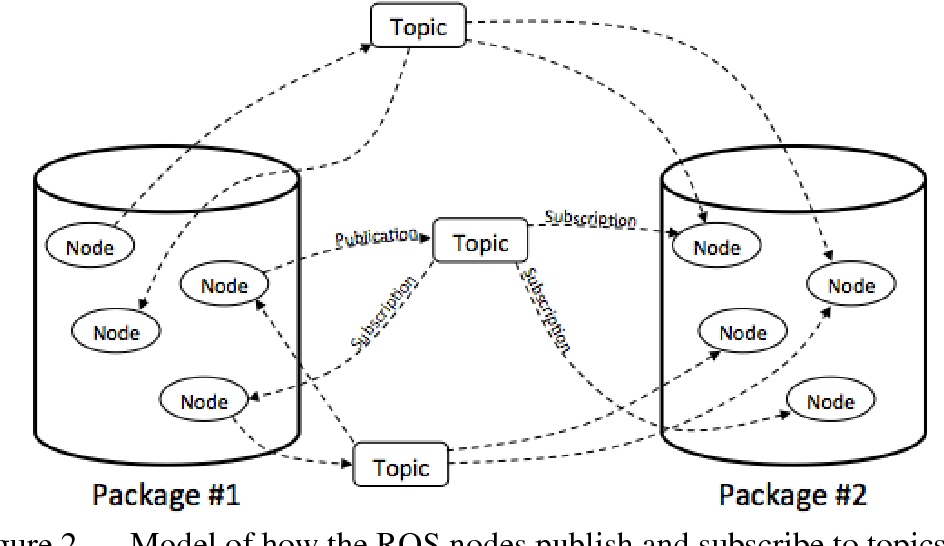
\includegraphics[width=0.9\linewidth]{Main/Chapter3/Images3/3-5/arquitectura-ros.png}
                \caption{Arquitectura por nodos de ROS}
                \label{f:Cap3-5_arquitectura_ros}
            \end{figure}
            
        \subsubsection{Orientación hacia las herramientas}
        
            Como lo demuestra la arquitectura duradera de Unix, se pueden crear sistemas de software complejos a partir de muchos programas pequeños y genéricos. A diferencia de muchos otros marcos de software de robótica, ROS no tiene un entorno de ejecución y desarrollo integrado canónico. Tareas como navegar por el árbol del código fuente, visualizar las interconexiones del sistema, trazar gráficamente los flujos de datos, generar documentación, registrar datos, etc, son todas realizadas por programas separados. Esto fomenta la creación de implementaciones nuevas y mejoradas, ya que (idealmente) se pueden intercambiar por implementaciones más adecuadas para un dominio de tarea en particular. Las versiones recientes de ROS permiten que muchas de estas herramientas se compongan en procesos únicos para mayor eficiencia o para crear interfaces coherentes para operadores o depuración, pero el principio sigue siendo el mismo: las herramientas individuales en sí mismas son relativamente pequeñas y genéricas.
            
        \subsubsection{Multilenguaje}
        
            Muchas tareas de software son más fáciles de realizar en lenguajes de secuencias de comandos de "alta productividad" como Python o Ruby. Sin embargo, hay ocasiones en las que los requisitos de rendimiento exigen el uso de lenguajes más rápidos, como C ++. También hay varias razones por las que algunos programadores prefieren lenguajes como Lisp o MATLAB. Se han librado guerras interminables de correo electrónico, se están librando actualmente y, sin duda, se seguirá librando sobre qué idioma es el más adecuado para una tarea en particular. Reconociendo que todas estas opiniones tienen mérito, que los lenguajes tienen diferentes utilidades en diferentes contextos, y que la experiencia única de cada programador es muy importante al elegir un idioma, ROS eligió un enfoque multilingüe. Los módulos de software ROS se pueden escribir en cualquier idioma para el que se haya escrito una biblioteca cliente. En el momento de escribir este artículo, existen bibliotecas cliente para C ++, Python, LISP, Java, JavaScript, MATLAB, Ruby, Haskell, R, Julia y otros. Las bibliotecas de cliente ROS se comunican entre sí siguiendo una convención que describe cómo los mensajes se ``aplanan'' o ``serializan'' antes de transmitirse a través de la red. Este libro utilizará la biblioteca cliente de Python casi exclusivamente, para ahorrar espacio en los ejemplos de código y para su facilidad de uso general. Sin embargo, las tareas descritas en este libro se pueden realizar con cualquiera de las bibliotecas cliente.
            
            \begin{figure}[htb]
                \centering
                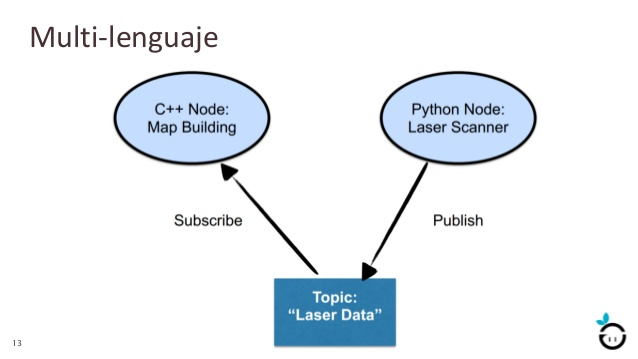
\includegraphics[width=0.9\linewidth]{Main/Chapter3/Images3/3-5/esquema-multi-lenguaje-ros.png}
                \caption{Esquema multilenguaje de ROS}
                \label{f:Cap3-5_multilenguaje_ros}
            \end{figure}
            
        \subsubsection{Pequeño}
        
            Las convenciones ROS alientan a los contribuyentes a crear bibliotecas independientes y luego empaquetar esas bibliotecas para que puedan enviar y recibir mensajes hacia y desde otros módulos ROS. Esta capa adicional está destinada a permitir la reutilización de software fuera de ROS para otras aplicaciones, y simplifica en gran medida la creación de pruebas automatizadas utilizando herramientas de integración continua estándar.
            
        \subsubsection{Libre y Open Source}
        
            El núcleo de ROS se publica bajo la licencia BSD permisiva, que permite el uso comercial y no comercial. ROS pas\subsua datos entre módulos mediante comunicación entre procesos (IPC), lo que significa que los sistemas construidos con ROS pueden tener licencias detalladas de sus diversos componentes. Los sistemas comerciales, por ejemplo, a menudo tienen varios módulos de fuente cerrada que se comunican con una gran cantidad de módulos de fuente abierta. Los proyectos académicos y de pasatiempos suelen ser de código abierto. El desarrollo de productos comerciales a menudo se realiza completamente detrás de un firewall. Todos estos casos de uso, y más, son comunes y perfectamente válidos bajo la licencia ROS.
            
            \begin{figure}[htb]
                \centering
                
\includegraphics[width=0.3\linewidth]{Main/Chapter3/Images3/3-5/licnecia-bsd-ros.png}
                \caption{Licencia de ROS}
                \label{f:Cap3-5_multilenguaje_ros}
            \end{figure}
            
        
            
    
        
    
        
    
    
       
       
\newpage

\section{Visualización}
    
    \subsection{Interfaz de visualización gráfica ROS visualization (Rviz)}

        RVIZ es la abreviación de ROS visualización. Es un entorno de visualización 3D de uso general para robots, sensores y algoritmos. Permite visualizar mapas, robots, objetos, datos láser, imágenes de cámaras, nubes de puntos y marcadores.   Como la mayoría de las herramientas ROS, se puede utilizar para cualquier robot y configurar rápidamente para una aplicación en particular.
        
        \begin{figure}[htb]
            \centering
            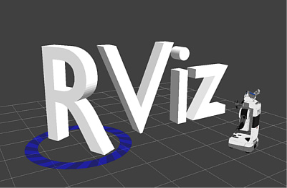
\includegraphics[width=0.5\linewidth]{Main/Chapter3/Images3/3-6/logo-rviz.png}
            \caption{Logo del software Rviz}
            \label{f:Cap3-6_logo_rviz}
        \end{figure}
        
        RVIZ proporciona una interfaz sencilla para elegir la información que queremos que se muestre. La Figura 3.2 muestra un ejemplo de la interfaz RVIZ. A la izquierda podemos ver todos los elementos que muestra RVIZ. Cada elemento debe configurarse con el nombre de un tema específico. Entonces RVIZ se suscribe a ese tema y visualiza su información. En el medio está la ventana principal donde se muestra toda la información y a la izquierda podemos elegir las propiedades de la herramienta y cambiar entre diferentes vistas. RVIZ también permite al usuario crear complementos para agregar nuevas capacidades de visualización.
        
        \begin{figure}[htb]
            \centering
            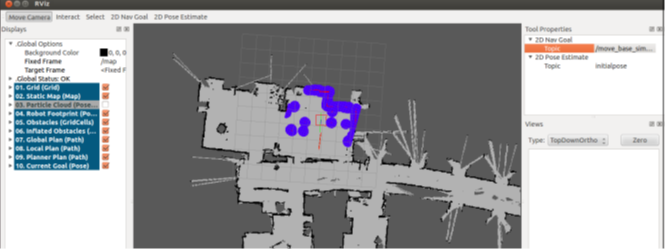
\includegraphics[width=0.8\linewidth]{Main/Chapter3/Images3/3-6/interfaz-rviz.png}
            \caption{Interfaz principal de Rviz}
            \label{f:Cap3-6_interfaz_rviz}
        \end{figure}
    
    \subsection{Interfaz de visualización gráfica ROS visualization (Rviz)}
    
        Un marco de coordenadas o frame es un concepto importante en ROS. Cualquier robot puede tener varios componentes, como un láser, una cámara, un sonar o brazos, y pueden tener un marco de coordenadas adjunto. Muchos algoritmos ROS requieren realizar un seguimiento de todos estos marcos de coordenadas.
        
        TF son las siglas en ingles de marco de transformadas (Transform frames) y es una de las librerías fundamentales de ROS. TF está diseñada para proporcionar una forma estándar de realizar un seguimiento de los marcos de coordenadas y transformar los datos dentro de todo el sistema a lo largo del tiempo. El paquete TF puede rastrear y mantener la relación entre múltiples marcos de coordenadas. Su función es proporcionar herramientas y funciones para definir todos los marcos de coordenadas de nuestro robot y transformar datos de un marco a otro, como por ejemplo puntos o vectores.
        
        \begin{figure}[htb]
            \centering
            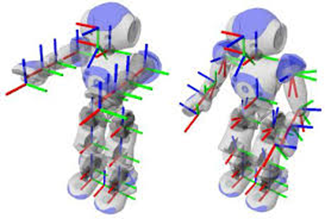
\includegraphics[width=0.8\linewidth]{Main/Chapter3/Images3/3-6/ejemplo-multiples-frames-rviz.png}
            \caption{Múltiples ``frames'' en Rviz}
            \label{f:Cap3-6_frames_rviz}
        \end{figure}
        
        La biblioteca tf opera en un sistema distribuido, por lo que la información correspondiente a los marcos de coordenadas de un robot está disponible para todos los componentes ROS en cualquier parte del sistema. Se crea una estructura de árbol con todos los marcos de coordenadas del sistema y todas las transformaciones se publican a través del tema “tf”.
      
        \begin{figure}[htb]
            \centering
            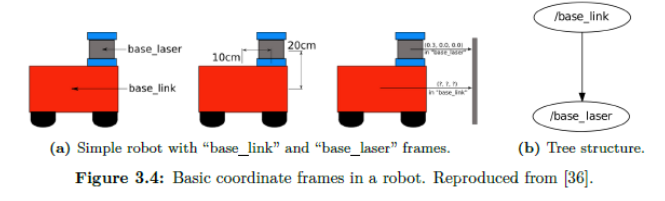
\includegraphics[width=0.8\linewidth]{Main/Chapter3/Images3/3-6/estructura-arbol-tf.png}
            \caption{nose}
            \label{f:Cap3-6_nose1}
        \end{figure}    
        
        Esta biblioteca tiene dos módulos estándar, broadcaster y listener. Estos módulos están diseñados para integrarse con el ecosistema ROS, pero generalmente son útiles fuera de ROS [20]. El broadcaster envía actualizaciones periódicamente de la pose de los fotogramas de coordenadas al resto del sistema. El sistema es capaz de tener muchos broadcaster que proporcionan información sobre una parte diferente del robot [19] [21]. El listener recopila los valores recibidos y almacena en búfer todos los fotogramas de coordenadas que se emiten en el sistema y consulta las transformaciones específicas entre fotogramas [21].

        \begin{figure}[htb]
            \centering
            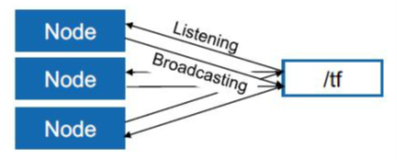
\includegraphics[width=0.8\linewidth]{Main/Chapter3/Images3/3-6/esquema-funcionamiento-tf.png}
            \caption{Ecosistema de la biblioteca TF}
            \label{f:Cap3-6_ecosistema_tf}
        \end{figure}   
        
        Además, TF ofrece una serie de herramientas o aplicaciones que facilitan al usuario la visualización del estado de las transformadas como:
        
        \begin{itemize}
            \item \textbf{tf\_monitor:} Imrpime la información sobre el árbol de transformación actual.
            \item \textbf{tf\_echo:} Imprime información sobre la transformación entre dos fotogramas.
            \item \textbf{tf\_tree:} Crea un gráfico visual del árbol de transformación (en formato pdf).
        \end{itemize}
        
        En la Figura \ref{f:Cap3-6_sistema_arbol_tf} se muestra un árbol de transformada haciendo uso de la herramienta rqt\_tf\_tree. En él se puede observar los distintos frames del sistema y sus relaciones
        
        \begin{figure}[htb]
            \centering
            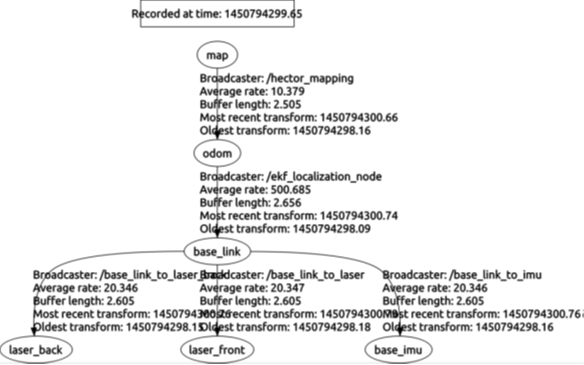
\includegraphics[width=1.0\linewidth]{Main/Chapter3/Images3/3-6/ejemplo-frames-sistema-arbol.png}
            \caption{Frames de un sistema visualizado mediante tf\_tree}
            \label{f:Cap3-6_sistema_arbol_tf}
        \end{figure} 
        
        \begin{figure}[htb]
            \centering
            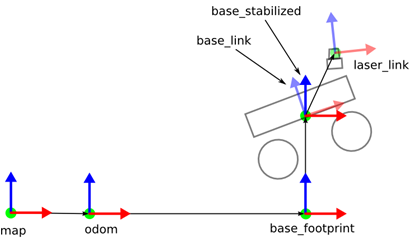
\includegraphics[width=1.0\linewidth]{Main/Chapter3/Images3/3-6/nose2.png}
            \caption{NO SE QUE ES}
            \label{f:Cap3-6_NOSE_tf}
        \end{figure} 
        
        Hay dos marcos de referencia que son importantes de conocer para obtener la visualización adecuada en Rviz:
        
        \begin{itemize}
            \item \textbf{Fixed frame:} Es el más importante de los dos. El fixed frame o marco fijo es el marco de referencia utilizado como frame global. Por norma general, este marco se suele asociar al mapa o ``mundo'' para poder visualizar los datos de manera correcta.
            \item \textbf{Target frame:} Es el sistema de coordenadas que sirve como referencia, por ejemplo, a la cámara o vista del visualizador, pudiendo tener distintas vistas e ir cambiando dependiendo de la perspectiva que se desee visualizar.
        \end{itemize}
        
        Resumiendo esta sección, TF es una biblioteca con las siguientes características:
        
        \begin{itemize}
            \item Es una herramienta para realizar un seguimiento de los marcos de coordenadas a lo largo del tiempo.
            \item Mantiene la relación entre los marcos de coordenadas en una estructura de árbol almacenada en el tiempo
            \item Permite al usuario transformar puntos y vectores entre marcos de coordenadas en cualquier momento deseado
            \item Es implementado como modelo de publisher/subscriber en los temas con nombres /tf y /tf\_statics
        \end{itemize}
        
        
    \subsection{Unified Robot Description Format (URDF)}\label{cap2_urfdf}
    
        \subsubsection{Introducción URDF}
    
        En ROS, es posible visualizar un modelo de un robot mediante el uso de archivos de formato de descripción de robot unificado (URDF). Sin embargo, solo aquellos robots que tienen eslabones rígidos conectados mediante articulaciones pueden ser descritos mediante modelos URDF.  Se puede usar un modelo URDF para calcular la cinemática, agregar nuevos marcos de coordenadas y moverlos de acuerdo con los valores del codificador del robot. Además, puede incluir otras propiedades físicas como inercia, colisiones, dinámica de articulaciones, etc. 
        
        Los archivos URDF están basados en XML y como tal, están compuestos por etiquetas de XML especiales que pueden ser leídas para extracción de información. A la lectura del archivo para extraer la información importante del modelo se denomina parsing y al programa o función que lo realiza, parser.
        
        La descripción del modelo consiste básicamente en de unir dos conjuntos: el conjunto de enlaces (link) y el conjunto de uniones (Joint). La forma de construir y visualizar un modelo de robot en URDF es escribir y compilar el archivo URDF. Una vez que se crea la representación 3D de un robot mediante el uso de un archivo URDF, es posible utilizar dicha representación para simular el movimiento del robot. Para ello, el usuario debe publicar las condiciones del robot en TF, utilizando un nodo (o nodos) para publicar la información de transformación [22].
        
        \begin{figure}[htb]
            \centering
            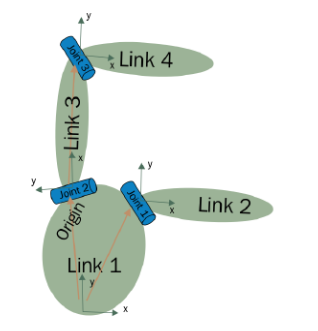
\includegraphics[width=1.0\linewidth]{Main/Chapter3/Images3/3-7/representacion-de-eslabon-en-urdf.png}
            \caption{Representación de un eslabón en URDF}
            \label{f:Cap3-7_eslabon_urdf}
        \end{figure} 
        
        \subsubsection{Links}
        
        El eslabones o enlaces (conjunto link) describen la parte física rígida del robot y permite especificar sus propiedades, como tamaño, forma, color o una malla 3D compleja importada. Consta de tres elementos:
    
        \begin{figure}[htb]
            \centering
            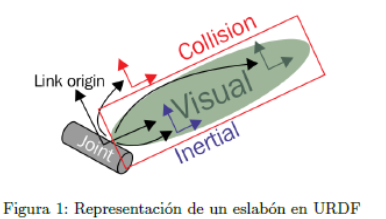
\includegraphics[width=1.0\linewidth]{Main/Chapter3/Images3/3-7/eslabon2.png}
            \caption{nose}
            \label{f:Cap3-7_noseee_urdf}
        \end{figure} 

        \begin{enumerate}
            \item \textbf{Inertial:} Especifica las propiedades inerciales del link (posición del centro de masas, la masa y la matriz Inercia)
            \item \textbf{Visual:} en este elemento viene especificado como debe estar representado el link. Es posible usar solidos simples como una esfera o un cilindro, o hacer representaciones más trabajadas como mallados o nube de puntos. Del mismo modo, también y se pueden definir los colores e importar texturas.
            \item \textbf{Collision:} Describe las propiedades de colisión de los links. Puede ser una forma diferente a la visual, como una figura más simple que sea representativa, a fin de reducir los tiempos de calculo en las simulaciones.
        \end{enumerate}
        
        \begin{figure}[htb]
            \centering
            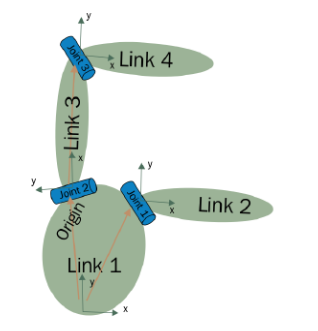
\includegraphics[width=1.0\linewidth]{Main/Chapter3/Images3/3-7/representacion-de-eslabon-en-urdf.png}
            \caption{Representación de un eslabón en URDF}
            \label{f:Cap3-7_eslabon_urdf}
        \end{figure} 
        
        
    
    
    \newpage

\section{Software Algorithm Development and mining (ADAMS)}
Desde

    
      
        
            
            
            

        
    
    